%----------------------------------------------------------------------------------------
%	PACKAGES AND OTHER DOCUMENT CONFIGURATIONS
%----------------------------------------------------------------------------------------

\documentclass[a0paper,portrait]{baposter}

\usepackage[font=small,labelfont=bf]{caption} % Required for specifying captions to tables and figures
\usepackage{booktabs} % Horizontal rules in tables
\usepackage{relsize} % Used for making text smaller in some places

%\usepackage[utf8]{inputenc} % Polish language
%\usepackage{polski} % Polish language
%\usepackage[polish]{babel} % Polish language
\newcommand*\rot{\rotatebox{90}}
\usepackage{array,multirow,graphicx}
\usepackage{wrapfig} % Wrapping table
\usepackage{colortbl}% http://ctan.org/pkg/xcolor % Color cells

\usepackage{wrapfig} % Putting QR code
\usepackage{multicol} % Make 3 columns of itemized genomes groups

%\usepackage{graphics,graphicx} % POA graph example drawing
%\usepackage{pstricks,pst-node,pst-tree} % POA graph example drawing
\usepackage{tikz}

\usepackage{url}
\graphicspath{{images/}} % Directory in which figures are stored

\definecolor{bordercol}{HTML}{1b0d13} % Border color of content boxes
\definecolor{headercol1}{HTML}{582719} % Background color for the header in the content boxes (left side)
\definecolor{headercol2}{HTML}{a5694b} % Background color for the header in the content boxes (right side)
\definecolor{headerfontcol}{HTML}{e7dcc8} % Text color for the header text in the content boxes
\definecolor{boxcolor}{HTML}{e6e8ea} % Background color for the content in the content boxes

\begin{document}

\background{ % Set the background to an image (background.pdf)
\begin{tikzpicture}[remember picture,overlay]
\draw (current page.north west)+(-2em,2em) node[anchor=north west]
{
\includegraphics[height=1.1\textheight]{background}};
\end{tikzpicture}
}

\begin{poster}{
grid=false,
borderColor=bordercol, % Border color of content boxes
headerColorOne=headercol1, % Background color for the header in the content boxes (left side)
headerColorTwo=headercol2, % Background color for the header in the content boxes (right side)
headerFontColor=headerfontcol, % Text color for the header text in the content boxes
boxColorOne=boxcolor, % Background color for the content in the content boxes
headershape=roundedright, % Specify the rounded corner in the content box headers
headerfont=\Large\sf\bf, % Font modifiers for the text in the content box headers
textborder=rectangle,
background=user,
headerborder=open, % Change to closed for a line under the content box headers
boxshade=plain
}
{}
%
%----------------------------------------------------------------------------------------
%	TITLE AND AUTHOR NAME
%----------------------------------------------------------------------------------------
%
{\sf\bf Pan-genome structural analysis and visualisation} % Poster title
{\vspace{1em} Paulina Dziadkiewicz, Jakub Tyrek, Norbert Dojer\\ % Author names
{\smaller pedziadkiewicz@gmail.com, jakubtyrek@gmail.com, dojer@mimuw.edu.pl}} % Author email addresses
{
\includegraphics[scale=0.6]{english_logo}} % University/lab logo

%----------------------------------------------------------------------------------------
%	INTRODUCTION
%----------------------------------------------------------------------------------------

\headerbox{Introduction}{name=introduction,column=0,row=0}{
Multiple sequence alignment is an information-rich object. Our aim is to analyze its component sequences by building a tree which consists of consensuses extracted from the alignment.\\ \\
A powerful way to achieve this result is to use graph representation of multiple alignment. It can be examined visually and be processed efficiently.
}

%----------------------------------------------------------------------------------------
%	GRAPH REPRESENTATION
%----------------------------------------------------------------------------------------

\headerbox{POA graph}{name=graph,column=0,below=introduction}{

\begin{description}
\item[Graph representation] of multiple alignment is based on partial order alignment graph (POA graph)\cite{lee02}. It reflects the multiple alignment structure in a more concise and intuitive way than typical approaches like MAF files or alignment browsers.
\end{description}
The basic idea is to merge aligned nucleotides which are the same into single nodes, create directed edges between subsequent nodes and undirected edges between aligned but different nucleotides.
\begin{center}
\texttt{CATCGATGA} \\
\texttt{GATG-TTGA} 
$$\downarrow$$
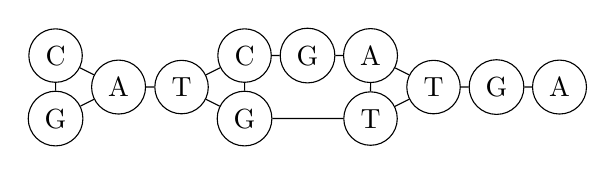
\begin{tikzpicture}
  [scale=.4,auto=left,every node/.style={circle,draw}]
  \node (n1) at (1,10) {C};
  \node (n2) at (1, 8) {G};
  \node (n3) at (3, 9) {A};
  \node (n4) at (5, 9) {T};
  \node (n5) at (7,10) {C};
  \node (n6) at (7, 8) {G};
  \node (n7) at (9,10) {G};
  \node (n8) at (11,10){A};
  \node (n9) at (11,8) {T};
  \node (n10) at (13,9) {T};
  \node (n11) at (15,9) {G};
  \node (n12) at (17,9) {A};
  
  \draw (n1) -> (n3);
  \draw (n2) -> (n3);
  \draw (n3) -> (n4);
  \draw (n4) -> (n5);
  \draw (n4) -> (n6);
  \draw (n5) -> (n7);
  \draw (n7) -> (n8);
  \draw (n6) -> (n9);
  \draw (n8) -> (n10);
  \draw (n9) -> (n10);  
  \draw (n10) -> (n11);
  \draw (n11) -> (n12);
  \draw (n1) -> (n2) [dashed];
  \draw (n5) -> (n6) [dashed];
  \draw (n8) -> (n9) [dashed];

\end{tikzpicture}
\end{center}

\begin{description}
\item[Consensus] in  a POA graph is a path representing some sequences present in the multialignment. By using heaviest bundle algorithm implemented in software called \textsl{poa}\cite{lee04} many consensuses can be defined.
\end{description}

}

%----------------------------------------------------------------------------------------
%	CONCLUSION
%----------------------------------------------------------------------------------------

\headerbox{Conclusion}{name=conclusion,column=0,below=graph}{
This work represents an approach to analyse \textbf{a pan-genome}. An insight into complex multialignments is given by \textbf{a tree of consensuses}. This is not only an attempt to reconstruct phylogenetic tree but also identification of sequences patterns shared by individuals and analysis of the alignment structure.\\
Enhancements planned to be undertaken are: a fast algorithm for handling cycles in genome graphs and visualization development.
}

%----------------------------------------------------------------------------------------
%	REFERENCES
%----------------------------------------------------------------------------------------

\headerbox{References}{name=references,column=0,below=conclusion}{

\smaller % Reduce the font size in this block

\renewcommand{\section}[2]{} % Get rid of the default "References" section title
\begin{thebibliography}{1}
\bibitem{lee02}
  Lee C., Grasso C., Sharlow M.F.
  \textit{Multiple sequence alignment using partial order graphs},
  Bioinformatics (2002) 18 (3): 452-464.
  
\bibitem{lee04}
  Lee C.
  \textit{Generating consensus sequences from partial order multiple sequence alignment graphs},
  Bioinformatics. (2003) 22;19(8):999-1008.
  
\bibitem{ebolaportal}
Haeussler et al. 
\textit{The UCSC Ebola Genome Portal.},
 PLOS Currents Outbreaks. 2014 Nov 7 . Edition 1.
 
\bibitem{mycoplasma}
\textit{Mycoplasma genomes phylogeny} \url{https://www.patricbrc.org/view/Taxonomy/2093#view_tab=phylogeny}, Accessed: April 2018
\end{thebibliography}
}

%----------------------------------------------------------------------------------------
%	ACKNOWLEDGEMENTS
%----------------------------------------------------------------------------------------

\headerbox{Acknowledgements}{name=acknowledgements,column=0,below=references, above=bottom}{
\smaller % Reduce the font size in this block
This work was supported by the National Science Centre, Poland, under grant number 2016/21/B/ST6/01471.} 


%----------------------------------------------------------------------------------------
%	TREE OF CONSENSUSES
%----------------------------------------------------------------------------------------

\headerbox{How to get the tree of consensuses?}{name=methods,span=2,column=1,row=0}{ % To reduce this block to 1 column width, remove 'span=2'

The tree of consensuses is being built in the top-down manner from the POA graph \textbf{G} representing the multiple sequence alignment. Given a \textbf{G}-subgraph \textbf{SG} reflecting sequences assigned to the current node, the following procedeure creates this node's children:

%Firstly, convert a multiple sequence alignment (eg. MAF file) into POA graph \textbf{G}. The consensuses tree is being built in a breadth first manner. In the following iterations, on the subsequent subgraphs \textbf{SG} of the original graph \textbf{G}, the procedure of consensus generation and sequences assignment is carried out:
\begin{center}
\begin{minipage}{0.49\linewidth}
\begin{enumerate}
\setlength\itemsep{0em}
\item Run consensus generation algorithm on the \textbf{SG} to get a consensus \textbf{C}
\item Choose the most compatible with \textbf{C} sequences from \textbf{SG} and generate a consensus \textbf{BestC} for them only.
\item Set group \textbf{S} of the most compatible with \textbf{BestC} \textbf{SG}-sequences.
\item Add \textbf{BestC} with sequences \textbf{S} to the consensuses tree and assign to it the minimum compatibility \textbf{Comp} to \textbf{BestC} among \textbf{S}.
\item Remove from \textbf{SG} sequences \textbf{S} and go to 1 if any sequences are left.
\item Re-assign sequences to \textbf{BestC} consensuses.
\end{enumerate}
\end{minipage}
\begin{minipage}{0.49\linewidth}
\begin{center}
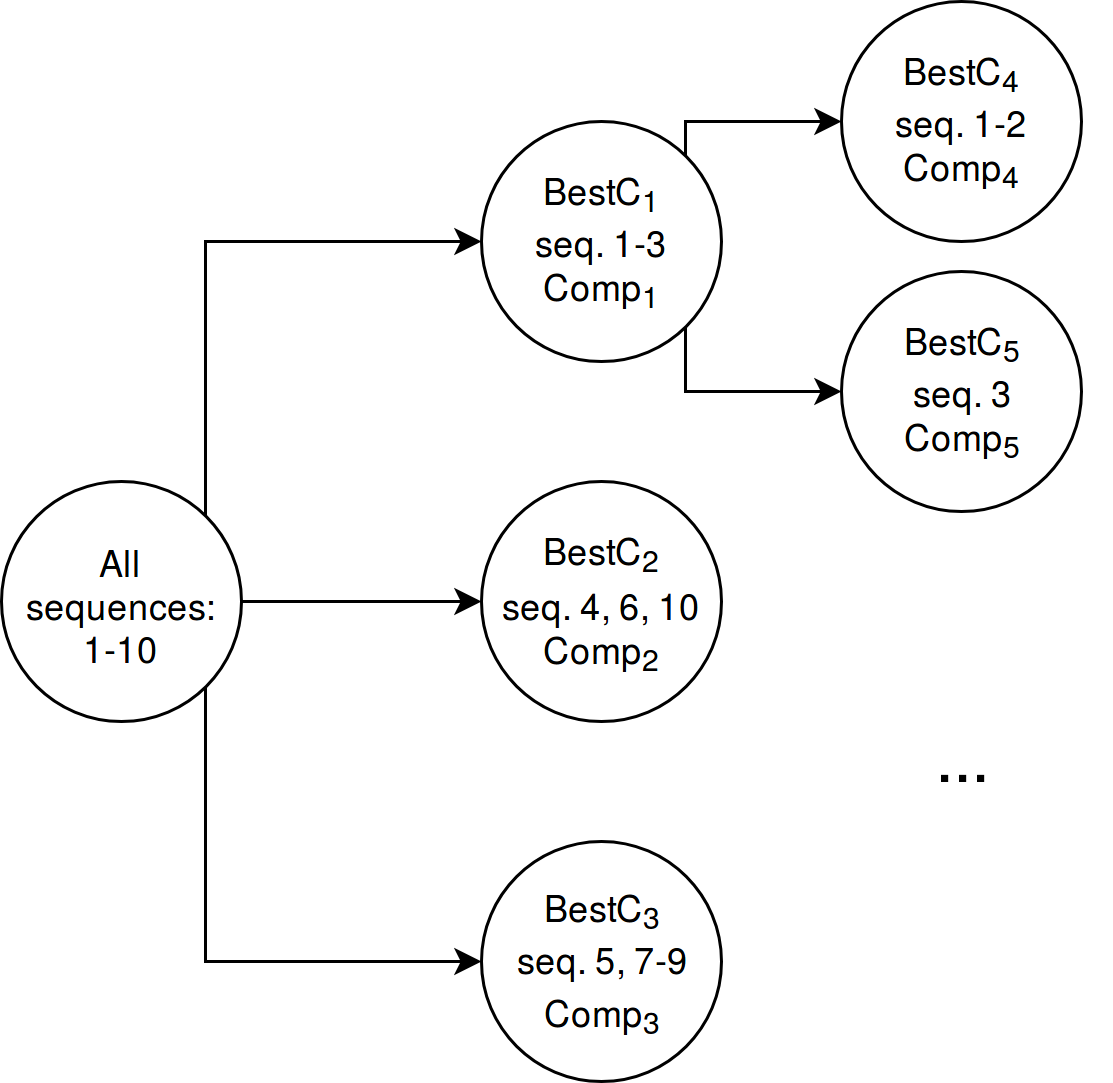
\includegraphics[scale=0.13]{consensuses_tree2}
\captionof{figure}{Tree of consensuses}
\end{center}
\end{minipage}
\end{center}

The above schema is used to split sequences into groups and assign a best consensus for them, until required level of fragmentation is reached.
}

%----------------------------------------------------------------------------------------
%	RESULTS EBOLA
%----------------------------------------------------------------------------------------

\headerbox{Results - Ebola}{name=results1,column=1,below=methods}{ % To reduce this block to 1 column width, remove 'span=2'
One dataset used in this research comes from USCB Ebola Portal \cite{ebolaportal}. There is a multiple alignment created for 158 Ebola and 2 Marburg viruses coming from all over the world, sequenced at different times. The received consensus tree is compatible with the biologically substantiated sequences division.

%The above solution was tested on two multiple alignments. One contains 159 genomes of the Ebola virus and the other one 7 genomes of the bacteria Mycoplasma (only a part of the genomes was used due to efficiency issues). The results were confronted with existing taxonomic databases \cite{ebolaportal}\cite{mycoplasma}.

%------------------------------------------------

\begin{center}
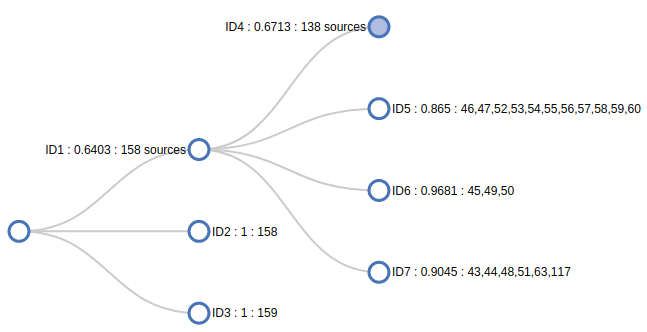
\includegraphics[width=1\linewidth]{ebola_tree}
\end{center}

}

%----------------------------------------------------------------------------------------

%----------------------------------------------------------------------------------------
%	RESULTS MYCOPLASMA
%----------------------------------------------------------------------------------------

\headerbox{Results - Mycoplasma}{name=results2,column=2,below=methods}{ % To reduce this block to 1 column width, remove 'span=2'
The other dataset was a multiple alignment built from 7 genomes of the bacteria Mycoplasma (M. pneumoniae, M. genitalium, M. gallisepticum). Only the part of the genomes could be used that satisfies POA graph requirement for being cycles-free.\\

The results were successfully confronted with existing taxonomic databases \cite{mycoplasma}.

%------------------------------------------------

\begin{center}
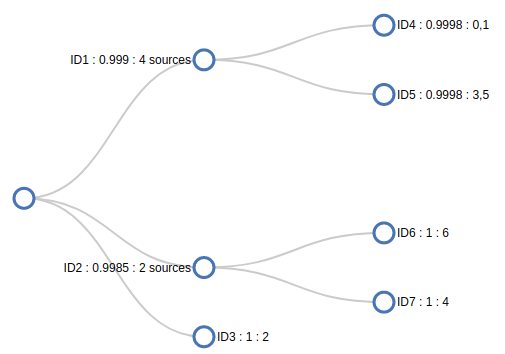
\includegraphics[width=0.5\linewidth]{mycoplasma_tree}
\end{center}


}

%----------------------------------------------------------------------------------------

%----------------------------------------------------------------------------------------
%	Visual representation
%----------------------------------------------------------------------------------------

\headerbox{Visual representation}{name=results2,span=2,column=1,below=results1,above=bottom}{ % To reduce this block to 1 column width, remove 'span=2'
The high-level purpose of the tool under development is pan-genome analysis and visualization.\\
Currently the visualization consists of:
\begin{itemize}
\item POA graph built from the multiple alignment which shows its structure on a nucleotides level
\item interactive tree of consensuses generated with the algorithm described above
\item tabular summary of sequences present in the alignment
\end{itemize}


\begin{center}
\begin{minipage}{0.49\linewidth}
\centering	
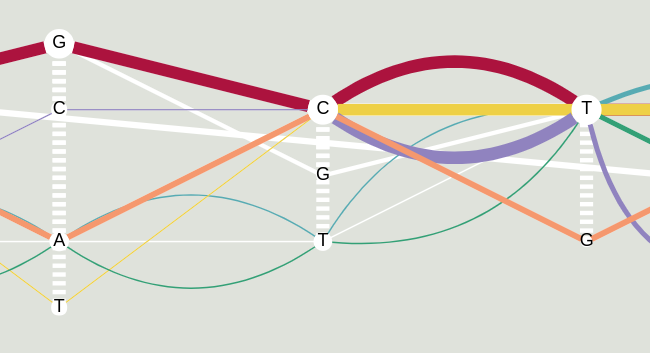
\includegraphics[width=1\linewidth]{ebola_100_cons}
\captionof{figure}{An excerpt of a POA graph.}
\end{minipage}
\begin{minipage}{0.49\linewidth}
\centering
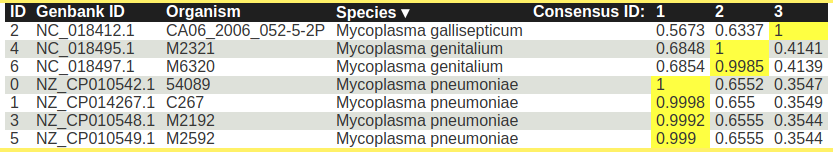
\includegraphics[width=1\linewidth]{mycoplasma_summary}
\captionof{figure}{Example sequences summary for Mycoplasma.}
\end{minipage}
\end{center}


}

\end{poster}

\end{document}
